\def\year{2021}\relax
%File: formatting-instructions-latex-2021.tex
%release 2021.2
\documentclass[letterpaper]{article} % DO NOT CHANGE THIS
\usepackage{aaai21}  % DO NOT CHANGE THIS
\usepackage{times}  % DO NOT CHANGE THIS
\usepackage{helvet} % DO NOT CHANGE THIS
\usepackage{courier}  % DO NOT CHANGE THIS
\usepackage[hyphens]{url}  % DO NOT CHANGE THIS
\usepackage{graphicx} % DO NOT CHANGE THIS
\urlstyle{rm} % DO NOT CHANGE THIS
\def\UrlFont{\rm}  % DO NOT CHANGE THIS
\usepackage{natbib}  % DO NOT CHANGE THIS AND DO NOT ADD ANY OPTIONS TO IT
\usepackage{caption} % DO NOT CHANGE THIS AND DO NOT ADD ANY OPTIONS TO IT
\frenchspacing  % DO NOT CHANGE THIS
\setlength{\pdfpagewidth}{8.5in}  % DO NOT CHANGE THIS
\setlength{\pdfpageheight}{11in}  % DO NOT CHANGE THIS
%\nocopyright
%PDF Info Is REQUIRED.
% For /Author, add all authors within the parentheses, separated by commas. No accents or commands.
% For /Title, add Title in Mixed Case. No accents or commands. Retain the parentheses.
\pdfinfo{
/Title (Domain-agnostic Outlier Ranking Algorithms (DORA)---A Configurable Pipeline for Facilitating Outlier Detection in Scientific Datasets)
/Author (AAAI Press Staff, Pater Patel Schneider, Sunil Issar, J. Scott Penberthy, George Ferguson, Hans Guesgen, Francisco Cruz, Marc Pujol-Gonzalez)
/TemplateVersion (2021.2)
} %Leave this
% /Title ()
% Put your actual complete title (no codes, scripts, shortcuts, or LaTeX commands) within the parentheses in mixed case
% Leave the space between \Title and the beginning parenthesis alone
% /Author ()
% Put your actual complete list of authors (no codes, scripts, shortcuts, or LaTeX commands) within the parentheses in mixed case.
% Each author should be only by a comma. If the name contains accents, remove them. If there are any LaTeX commands,
% remove them.

% DISALLOWED PACKAGES
% \usepackage{authblk} -- This package is specifically forbidden
% \usepackage{balance} -- This package is specifically forbidden
% \usepackage{color (if used in text)
% \usepackage{CJK} -- This package is specifically forbidden
% \usepackage{float} -- This package is specifically forbidden
% \usepackage{flushend} -- This package is specifically forbidden
% \usepackage{fontenc} -- This package is specifically forbidden
% \usepackage{fullpage} -- This package is specifically forbidden
% \usepackage{geometry} -- This package is specifically forbidden
% \usepackage{grffile} -- This package is specifically forbidden
% \usepackage{hyperref} -- This package is specifically forbidden
% \usepackage{navigator} -- This package is specifically forbidden
% (or any other package that embeds links such as navigator or hyperref)
% \indentfirst} -- This package is specifically forbidden
% \layout} -- This package is specifically forbidden
% \multicol} -- This package is specifically forbidden
% \nameref} -- This package is specifically forbidden
% \usepackage{savetrees} -- This package is specifically forbidden
% \usepackage{setspace} -- This package is specifically forbidden
% \usepackage{stfloats} -- This package is specifically forbidden
% \usepackage{tabu} -- This package is specifically forbidden
% \usepackage{titlesec} -- This package is specifically forbidden
% \usepackage{tocbibind} -- This package is specifically forbidden
% \usepackage{ulem} -- This package is specifically forbidden
% \usepackage{wrapfig} -- This package is specifically forbidden
% DISALLOWED COMMANDS
% \nocopyright -- Your paper will not be published if you use this command
% \addtolength -- This command may not be used
% \balance -- This command may not be used
% \baselinestretch -- Your paper will not be published if you use this command
% \clearpage -- No page breaks of any kind may be used for the final version of your paper
% \columnsep -- This command may not be used
% \newpage -- No page breaks of any kind may be used for the final version of your paper
% \pagebreak -- No page breaks of any kind may be used for the final version of your paperr
% \pagestyle -- This command may not be used
% \tiny -- This is not an acceptable font size.
% \vspace{- -- No negative value may be used in proximity of a caption, figure, table, section, subsection, subsubsection, or reference
% \vskip{- -- No negative value may be used to alter spacing above or below a caption, figure, table, section, subsection, subsubsection, or reference

\setcounter{secnumdepth}{0} %May be changed to 1 or 2 if section numbers are desired.

\usepackage{siunitx}
\usepackage{amsmath}
\usepackage[dvipsnames]{xcolor}
\newcommand{\todo}[1]{\textcolor{blue}{#1}}

% The file aaai21.sty is the style file for AAAI Press
% proceedings, working notes, and technical reports.
%

% Title

% Your title must be in mixed case, not sentence case.
% That means all verbs (including short verbs like be, is, using,and go),
% nouns, adverbs, adjectives should be capitalized, including both words in hyphenated terms, while
% articles, conjunctions, and prepositions are lower case unless they
% directly follow a colon or long dash
\iffalse
\title{Domain-agnostic Outlier Ranking Algorithms (DORA)---A Configurable Pipeline for Facilitating Outlier Detection in Scientific Datasets}
\author{
    %Authors
    % All authors must be in the same font size and format.
    Written by AAAI Press Staff\textsuperscript{\rm 1}\thanks{With help from the AAAI Publications Committee.}\\
    AAAI Style Contributions by Pater Patel Schneider,
    Sunil Issar,  \\
    J. Scott Penberthy,
    George Ferguson,
    Hans Guesgen,
    Francisco Cruz,
    Marc Pujol-Gonzalez
    \\
}
\affiliations{
    %Afiliations
    \textsuperscript{\rm 1}Association for the Advancement of Artificial Intelligence\\
    %If you have multiple authors and multiple affiliations
    % use superscripts in text and roman font to identify them.
    %For example,

    % Sunil Issar, \textsuperscript{\rm 2}
    % J. Scott Penberthy, \textsuperscript{\rm 3}
    % George Ferguson,\textsuperscript{\rm 4}
    % Hans Guesgen, \textsuperscript{\rm 5}.
    % Note that the comma should be placed BEFORE the superscript for optimum readability

    2275 East Bayshore Road, Suite 160\\
    Palo Alto, California 94303\\
    % email address must be in roman text type, not monospace or sans serif
    publications21@aaai.org

    % See more examples next
}
\fi
\iffalse
%Example, Single Author, ->> remove \iffalse,\fi and place them surrounding AAAI title to use it
\title{My Publication Title --- Single Author}
\author {
    % Author
    Author Name \\
}

\affiliations{
    Affiliation \\
    Affiliation Line 2 \\
    name@example.com
}
\fi


%Example, Multiple Authors, ->> remove \iffalse,\fi and place them surrounding AAAI title to use it
\title{Domain-agnostic Outlier Ranking Algorithms (DORA)---A Configurable Pipeline for Facilitating Outlier Detection in Scientific Datasets}
\author {
    % Authors
    Hannah Kerner,\textsuperscript{\rm 1}
    Umaa Rebbapragada, \textsuperscript{\rm 2}
    Kiri Wagstaff, \textsuperscript{\rm 2} 
    Steven Lu, \textsuperscript{\rm 2} 
    Bryce Dubayah, \textsuperscript{\rm 1} \\
    Eric Huff, \textsuperscript{\rm 2} 
    Jake Lee, \textsuperscript{\rm 2} 
    Vinay Raman, \textsuperscript{\rm 3}
    Sakshum Kulshrestha \textsuperscript{\rm 1}  \\
}
\affiliations {
    % Affiliations
    \textsuperscript{\rm 1} University of Maryland, College Park \\
    \textsuperscript{\rm 2} Jet Propulsion Laboratory, 
    									   California Institute of Technology \\
    \textsuperscript{\rm 3} Montgomery Blair High School \\
    hkerner@umd.edu, \{umaa.d.rebbapragada,
    										kiri.l.wagstaff,
    										you.lu,
    										eric.m.huff,
    										jake.h.lee\}@jpl.nasa.gov
}

\begin{document}

\maketitle

\begin{abstract}
Automatic detection of outliers is
universally needed when working with scientific datasets, e.g., for cleaning 
datasets or flagging novel samples to guide instrument acquisition or
 scientific analysis.
We present Domain-agnostic Outlier Ranking Algorithms (DORA),
a configurable pipeline that facilitates application and evaluation of
outlier detection methods in a variety of domains. DORA allows users to 
configure experiments by specifying the location of their 
dataset(s), the input data type, feature extraction methods, and which 
algorithms should be applied. DORA supports image, raster, time series, 
or feature vector input data types and outlier detection methods that include
 Isolation Forest, DEMUD, PCA, RX detector, 
 Local RX, negative sampling, and probabilistic autoencoder. Each algorithm assigns an outlier score to each data sample. DORA
   provides results interpretation modules to help users 
   process the results, including sorting samples by outlier score, evaluating 
   the fraction of known outliers in $n$ selections, clustering groups of 
   similar outliers together, and web visualization. We demonstrated how DORA
   facilitates application, evaluation, and interpretation of outlier detection
   methods by performing
    experiments for three real-world datasets from Earth science, planetary
  science, and astrophysics, as well as one benchmark dataset 
  (MNIST/Fashion-MNIST). We found that no single algorithm
      performed best across all datasets, underscoring the need for a tool 
      that enables comparison of multiple algorithms.
\end{abstract}

\section{Introduction}
The ability to automatically detect out-of-distribution samples in large data 
sets is of interest for a wide variety of scientific domains. Depending on the
 application setting, this capability is also commonly referred to as anomaly
  detection, outlier detection, or novelty detection. More broadly, this is 
  referred to as out-of-distribution (OOD) detection. In general, the goal of 
  OOD detection systems is to identify samples that deviate from the majority
   of samples in a dataset in an unsupervised manner~\cite{pimentel2014review}. 
   In machine learning, these methods are commonly used for identifying 
   mislabeled or otherwise invalid samples in a dataset. When working with science datasets, OOD detection can be used for 
   cleaning datasets, e.g., flagging ground-truth labels with GPS or human
    entry error or identifying wrongly categorized objects in a catalog. 
    It could also be used for discovery, e.g., to flag novel samples in order 
    to guide instrument acquisition or scientific analysis. Another application
   is the detection of rare objects that are known to exist but the known
   examples are too few to create a large enough labeled dataset for 
   supervised classification algorithms. 
   
  Despite wide differences in applications, data types, and dimensionality,
 the same underlying machine learning algorithms can be employed across 
 all of these domains. A challenge for applying them however is that domain
 scientists do not always have the programming or machine learning background
 to apply the algorithms themselves using existing tools. Given the widespread 
 applicability and transferability of OOD methods, the scientific community 
 would benefit from a tool that made it easy for them to apply popular outlier
 detection algorithms to their science datasets. We created DORA 
 (Domain-agnostic Outlier Ranking Algorithms) 
 to provide a tool for applying outlier 
 detection algorithms to a variety of scientific data sets with minimal coding
 required. Users need only to specify details for their data/application 
 including the data type, location, and algorithms to run in an experiment
 configuration file. DORA supports image, raster, time series, 
or feature vector input data types and outlier detection methods that include
 Isolation Forest, Discovery via Eigenbasis Modeling of Uninteresting Data 
 (DEMUD)~\citep{wagstaff:demud13}, principal component analysis (PCA),
   Reed-Xiaoli (RX) detector,  
 Local RX, negative sampling~\cite{sipple:neg-sampling20}, and probabilistic 
 autoencoder (PAE). 
 Each algorithm assigns an outlier 
 score to each sample in a given dataset. 
 DORA provides results organization and visualization 
 modules to help users process the results, including sorting samples by outlier 
 score, evaluating outlier recall for a set of known/labeled outliers, clustering 
 groups of similar outliers together, and web visualization. 
 We demonstrated how DORA
   facilitates application, evaluation, and interpretation of outlier detection
   methods by performing
    experiments for three real-world datasets from Earth science, planetary
  science, and astrophysics, as well as one benchmark dataset 
  (MNIST/Fashion-MNIST). We found that no single algorithm
      performed best across all datasets, underscoring the need for a tool 
      that enables comparison of multiple algorithms.

\section{Related Work}
Methods for outlier detection have been 
surveyed extensively and can be differentiated primarily based on how they 
score outliers
~\cite{pimentel2014review,chandola2009anomaly,markou2003novelty,
markou2003novelty2}.
%
Reconstruction-based methods construct a model of a dataset by learning 
a mapping between the input data and a lower-dimensional representation that
 minimizes the loss between the input and its reconstruction from the 
 low-dimensional representation~\citep{kerner2020comparison}. The 
 reconstruction error is used as the outlier score because samples
  that are unlike the data used to fit the model will be more poorly 
  reconstructed compared to inliers. Reconstruction-based methods
  include PCA~\cite{jablonski2015principal}, 
  autoencoders~\cite{richter2017safe}, and
  generative adversarial networks~\cite{akcay2018ganomaly}.
%
 Distance-based methods score outliers based on their distance from a
``background'' which can be defined in a variety of ways. For example,
the Reed-Xiaoli (RX) detector computes the 
Mahalanobis distance between each sample and the background dataset
defined by its mean and covariance matrix~\cite{reed1990adaptive}.
%
Sparsity-based methods such as isolation forest~\cite{liu2008isolation}
and local outlier factor~\cite{breunig2000lof}
 score outliers based on how isolated or sparse samples 
are in a given feature space. 
%
Probability distribution and density based methods estimate the underlying 
distribution or probability density of a dataset and score samples using
 likelihood. Examples include the probabilistic
autoencoder, which scores samples based on the log likelihood under the 
latent space distribution~\cite{bohm2020probabilistic}, Gaussian mixture 
Models, and kernel density estimators~\cite{chandola2009anomaly}. 
%
Other methods formulate outlier detection as supervised classification, 
usually with only one class constituted by 
known normal samples.
Such methods include one-class support vector 
machines~\cite{scholkopf1999support}
and negative sampling~\cite{sipple:neg-sampling20}.

In astrophysics, 
outlier detection methods have been used to identify astrophysical
objects with unique characteristics~\cite{hayat2021self} 
as well as data or modeling 
artifacts in astronomical surveys~\citep{wagstaff:des-anom20}. 
Example outlier detection applications in 
Earth science include detecting anomalous objects or materials
~\cite{zhou2016novel}, data artifacts or noise 
~\cite{liu2017unsupervised}, change~\cite{touati2020anomaly}, 
and ocean extremes~\cite{prochaska2021deep}. 
Planetary science applications have mostly focused 
on prioritizing samples with novel geologic or geochemical features for
follow-up targeting or analysis~\cite{kerner2020comparison,
wagstaff:demud13}.
%
These examples show the benefit of applying outlier detection methods in
a variety of real-world science use cases. However, the effort required to 
apply and evaluate the many available algorithms is non-trivial and can 
be daunting for non-ML experts, thus impeding the uptake of outlier
detection methods in science applications.  
There is a need for tools that make it easier for domain scientists to apply
outlier detection methods as well as compare results across datasets.
While there have been some efforts to develop tools for facilitating the
application of outlier detection methods~\cite{zhao2019pyod}, they cover
limited data formats and algorithms. DORA aims to fill the need 
for tools that faciliate application, evaluation, and interpretation of outlier
detection methods.

\section{Methods}
%\subsection{DORA configurable pipeline} 
Figure \ref{fig:dora} illustrates the architecture of DORA including 
data loading, feature extraction, outlier ranking, and results organization
and visualization modules. 
In order to improve the readability and execution speed of the code, we adopted
object-oriented and functional programming practices.  We designed DORA to be 
readily extensible to support additional data types or formats, outlier detection 
algorithms, and results organization or visualization methods by writing new 
modules that follow the DORA API. Experimental settings are controlled by 
configuration files in which users can specify the input data, 
feature extraction methods, normalization method, outlier ranking methods, and 
results organization methods. 
DORA is implemented in Python 3.

\paragraph{Data types.} We chose to implement data loaders for four
data types that are commonly used by the machine learning and domain science
communities: time series, feature vectors, images (grayscale or RGB), and 
$N$-band rasters. $N$-band rasters are images or grids in which every pixel
is associated with a location (e.g., latitude/longitude in degrees); 
most satellite data are distributed as rasters.
A data loader for each data type locates the data by the path(s)
defined in the configuration file and loads samples into a dictionary of numpy
 arrays indexed by the sample id. This \texttt{data\_dict} is then passed to each of the ranking algorithms.

\paragraph{Outlier ranking algorithms.} We implemented 7 unsupervised 
algorithms for scoring and 
ranking samples by outlierness. 
We chose these algorithms to include a diverse
set of approaches to scoring outliers since different algorithms may  
perform better for different datasets and use cases. 
%We describe each
%approach to scoring outliers and the associated methods below.

\begin{figure}
    \centering
    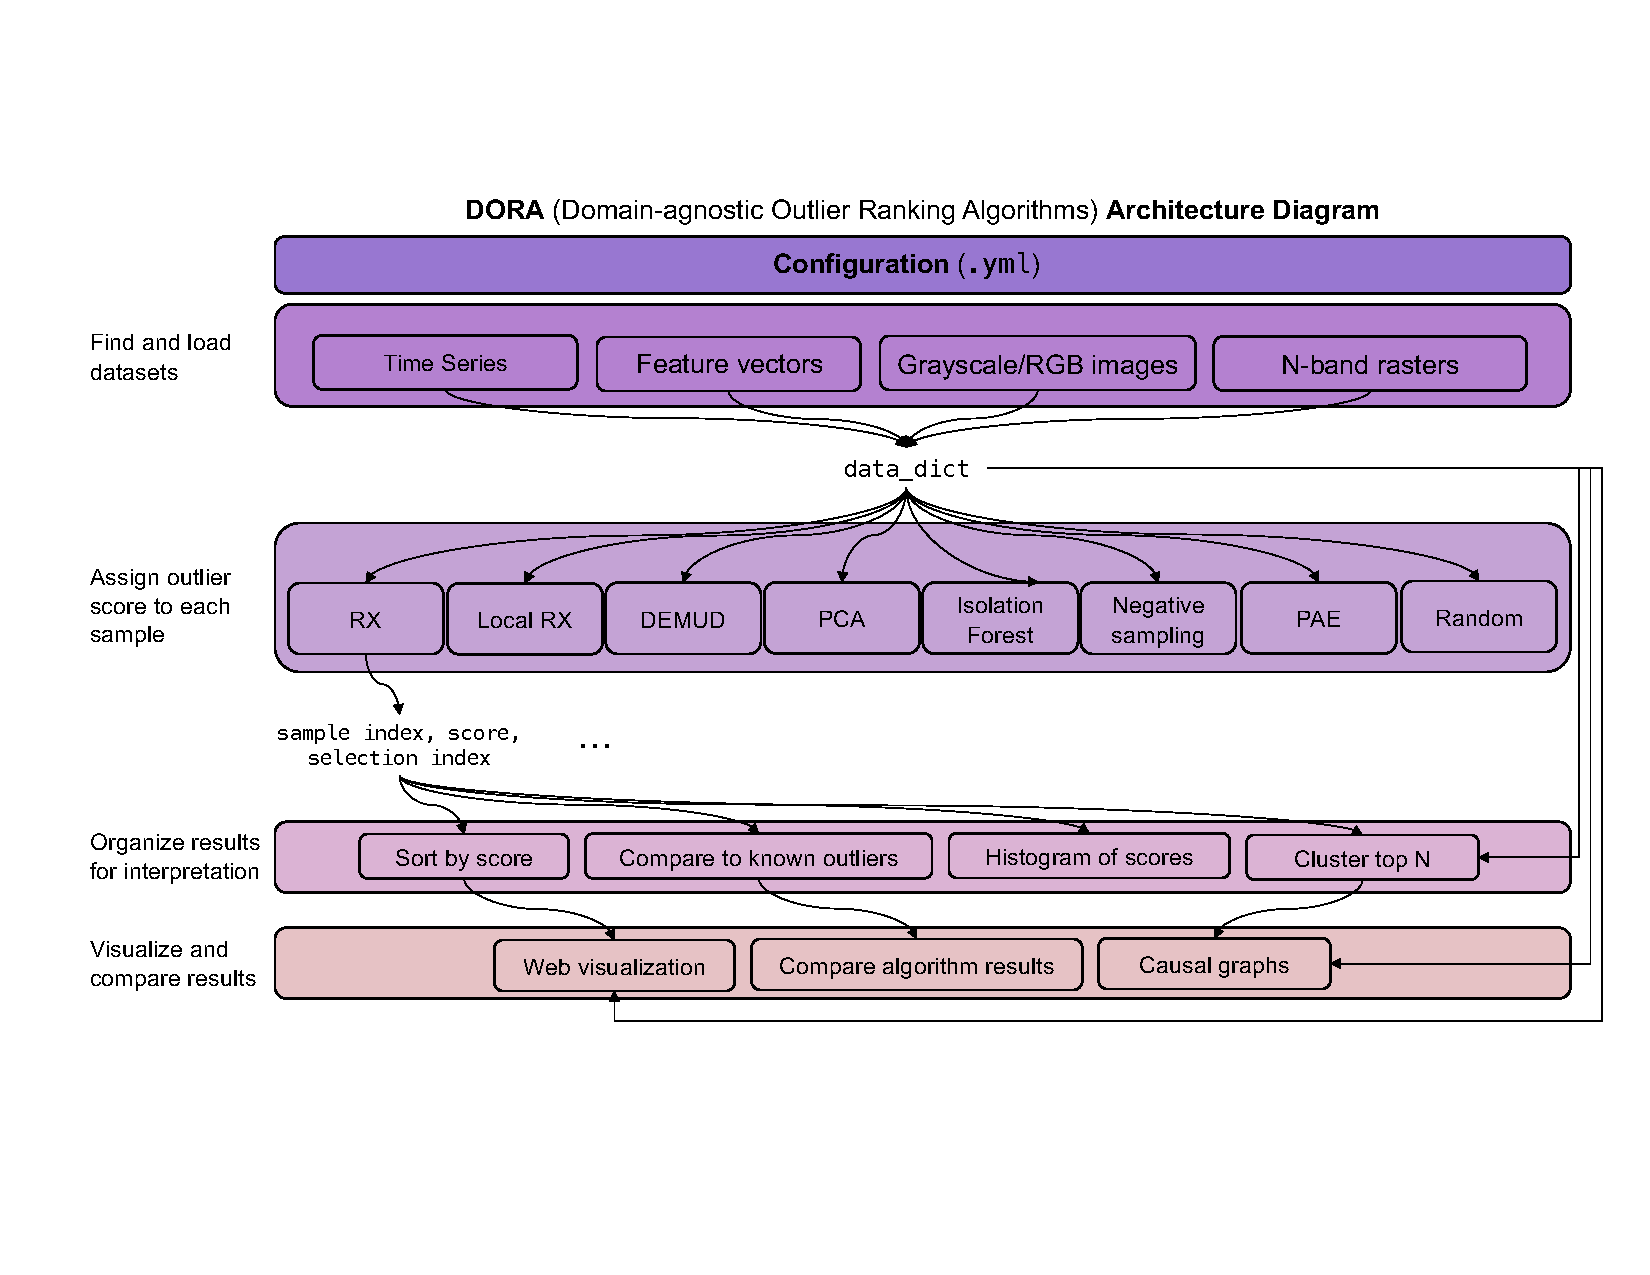
\includegraphics[width=\linewidth]{figures/dora-system-diagram-v5.pdf}
    \caption{DORA pipeline architecture.}
    \label{fig:dora}
\end{figure}

\subparagraph{Reconstruction error.}
Principal component analysis (PCA) has been used for outlier detection by
scoring samples using the reconstruction error (here, the L2 norm)
between inputs and their inverse
 transformation from the principal subspace~\citep{kerner2020comparison}.
 DEMUD~\citep{wagstaff:demud13} differs from other
outlier ranking methods: instead of independently scoring all
observations, DEMUD incrementally identifies the most unusual
remaining item, then incorporates it into the model of ``known''
(non-outlier) observations before selecting the next most unusual
item.  DEMUD's goal is to identify diverse outliers and avoid
redundant selections.  Once an outlier is found, repeated
occurrences of that outlier are deprioritized.  Methods that score
samples independently maximize coverage of outliers, while DEMUD
maximizes fast discovery of distinct outlier types.

\subparagraph{Distance.}
 The 
Reed-Xiaoli (RX) detector is commonly used for anomaly detection in
multispectral and hyperspectral remote sensing. RX scores samples using
 the Mahalanobis
 distance between a sample and a background mean and covariance
 ~\citep{reed1990adaptive}. The local variant of RX (Local
 RX or LRX) can be used for image or raster data and scores each pixel in
  an image with respect to a window ``ring'' of pixels surrounding 
  it~\citep{molero2013analysis}. 
  LRX requires two parameters to define the size of the outer window 
  surrounding the pixel and the inner window
   around the target pixel to exclude from the background distribution. 

\subparagraph{Sparsity.}
Isolation forests are a common sparsity-based method
that constructs many random binary trees from a 
dataset~\cite{liu2008isolation}. The outlier score for
a sample is quantified as the average distance from the root to the item’s 
leaf. Shorter distances are indicative of outliers because fewer splits were 
required to isolate the sample.

\subparagraph{Probability.}
The negative sampling algorithm is implemented by converting the unsupervised 
outlier ranking problem into a semi-supervised 
problem~\citep{sipple:neg-sampling20}. Negative (anomalous) 
examples are created by sampling from an expanded space defined by the minimum 
and maximum values of each dimension of the positive (normal) examples. The 
negative and positive examples are then used to train a random forest 
classifier. We use the posterior probabilities of the random forest classifier 
as outlier scores, which means that the observations with higher posterior 
probabilities are more likely to be outliers.
The probabilistic autoencoder is a generative model consisting of an
autoencoder trained to reconstruct input data which is interpreted
probabilistically after training using a normalizing flow on the autoencoder
latent space~\cite{bohm2020probabilistic}.
Samples are scored as outliers using the log likelihood in the latent
distribution, the autoencoder reconstruction error, or a combination of
both.

\paragraph{Results interpretation.}
Each of the outlier ranking algorithms returns an array containing the sample
index, outlier score, and selection index (index after sorting
by outlier score). DORA provides organization and visualization modules
intended to help users interpret and make decisions based on these outputs.
The simplest
 module saves a CSV of the samples sorted by their outlier score 
 (i.e., selection order). Clustering the top
  $N$ outlier selections can enable users to investigate the different types of 
 outliers that might be present in the dataset; this could be especially useful
 for separating outliers caused by noise or data artifacts vs. scientifically 
 interesting samples. We implemented the K-means and self-organizing maps 
 (SOMs) algorithms for clustering the top-N outliers. For use cases in which an
 evaluation dataset containing known outliers is available, we provide a module
 to assess how well algorithm selections correlate with known outliers. This is
 done by plotting the number of known outliers vs. number of selections made. 
We provide a module for plotting histograms of outlier scores to visualize the
 distribution of scores in the dataset (which may be, e.g., multimodal or 
 long-tailed). 
We developed a desktop application to easily visualize DORA results with the
Electron application framework and React frontend library. 
This enables fast and easy comparison of the results from
different methods. Figure \ref{fig:doravis} shows a screenshot of the
``Aggregate Table'' view, which displays all algorithm results 
side-by-side.

%We developed a desktop application to easily visualize DORA results with the
%Electron application framework and React frontend library. The application loads
%the DORA configuration file to locate the dataset and result CSVs. Then,
%it displays the ranked samples and their scores in a table sorted by their
%selection order. This allows for fast and easy comparison of the results of
%different methods. Figure \ref{fig:doravis} shows a screenshot of the
%``Aggregate Table'' view, which displays all results from different algorithms
%side-by-side.

\begin{figure}
  \centering
  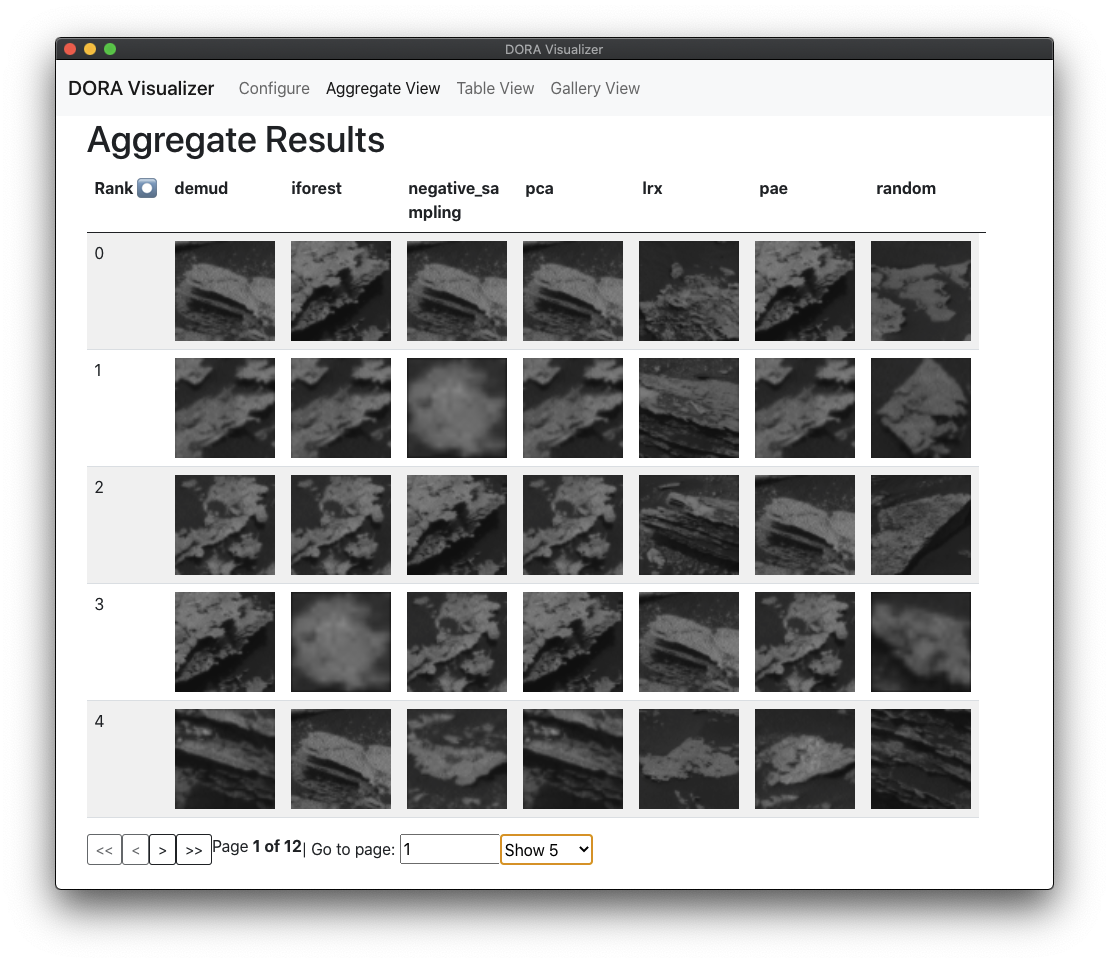
\includegraphics[width=0.83\linewidth]{figures/doravis.png}
  \caption{A screenshot of the DORA visualizer displaying results from the
  planetary science dataset.}
  \label{fig:doravis}
\end{figure}

\section{Datasets}
We constructed three datasets to evaluate the utility of DORA and 
algorithm performance for a variety of scientific domains
 (astrophysics, planetary science, and Earth science). We also included a 
 benchmark dataset that uses MNIST and Fashion-MNIST. Table \ref{tab:datasets}
 summarizes the number of unlabeled samples used for training evaluation for
 each dataset. We describe each dataset in detail below.
 
 \begin{table}
  \caption{Number of samples in the training and test sets for each dataset,
  ordered by dataset size.}
  \label{tab:datasets}
  \centering
  \begin{tabular}{l|c|cc}
    \hline
    Dataset & Training & \multicolumn{2}{c}{Test}\\
     & Unlabeled &  Outliers &  Inliers \\
    
    \hline
    Planetary & 992 &  9 & 49 \\
    Earth & 6,757 & 37 & 76  \\
    F-MNIST & 60,000 & 1,000 & 1,000  \\
    Astrophysics & 100,000   &  25,339 &  74,661 \\
    \hline
  \end{tabular}
\end{table}

\subsubsection{Astrophysics: objects in Dark Energy Survey.}
Astronomical data sets are large and growing. Large modern optical
imaging surveys are producing catalogs of order $10^8$ stars
and galaxies, with dozens or hundreds of distinct measured features
for each entry. Discovery science becomes difficult at this data
volume: the scale is too large for expert human inspection, and separating real
astrophysical anomalies from non-astrophysical sources like detector artifacts or
satellite trails is a challenging problem for current methods.

The Dark Energy Survey (DES) is an ongoing imaging survey of
$5000~{\rm deg}^2$ of the southern sky from the Cerro-Tololo
Inter-American Observatory in Chile~\cite{zuntz2018dark}. The resulting galaxy catalogs produced have provided some of the strongest constraints to date on
the physical properties of dark energy and accelerated expansion
of the Universe. The first version of this catalog, released June 2018, incorporated
only cuts on signal-to-noise and resolution, masks against known detector
anomalies and data quality indicators, and the automated data quality
flags produced during processing to filter outliers. 
In December 2019, the full catalog
was released after 18 months of extensive manual vetting. We used the samples 
that were removed in the second version of the catalog as a set of known
outliers for evaluating anomaly detection methods on the first version.

We compared all methods on a dataset of 100K galaxy objects
observed by the Dark Energy Survey (DES) sampled from the initial June 2018 release.
We labeled the 25,339 objects from this 100K set that did not appear in the later December 2019
release, thus were likely eliminated during the manual vetting process, 
as outliers.
While the remaining 74,661 objects may also contain outliers, we assume them to be inliers in this experiment. We used publicly-available photometry from the $g-$, $r-$, $i-$ and $z-$band DES exposures.  We
transformed the photometry into luptitudes\footnote{A
  ``Luptitude''~\cite{lupton99} is an arcsinh-scaled flux, with
  properties quantitatively equal to
  traditional astronomical magnitudes for bright sources, but which
  gracefully handles non-detections and negative fluxes.}.  The input features 
  were the $r$-band luptitude, colors computed as band differences between
$g-r$, $i-r$, and $z-r$, and associated observational errors, for a total of eight features.
%


\subsubsection{Planetary: targets in Mars rover images.}
Mars exploration is fundamentally an exercise in discovery with the
goal of increasing our understanding of Mars's history, evolution,
composition, and currently active processes.  Outliers
identified in Mars observations can inspire new discoveries and inform
the choice of which areas merit follow-up or deeper
investigation~\cite{kerner2020comparison,wagstaff:rover-novelty20}.
We collected \num{72} images from the Navigation camera (Navcam) 
on the Mars Science Laboratory (MSL) rover
and employed Rockster~\cite{burl:rockster16}
(currently used by onboard rover software) to identify candidate rock
targets with an area of at least 100 pixels, yielding \num{1050}
targets.  We cropped out a \num{64}$\times$\num{64} pixel image
centered on each target.

We simulated the operational setting in which the rover has observed
targets up through mission day (sol) $s$ and the goal is to rank all
subsequent targets (after sol $s$) to inform which recent targets
merit further study.  Our rover image data covers sols \num{1343}
to \num{1703}.  We partitioned the images chronologically to assess
outlier detection in the 10 most recent sols, using ``prior'' set
$D_{1343-1693}$ ($n=992$) and ``assessment'' set $D_{1694-1703}$
($n=58)$ for evaluation. We collaborated with an MSL science team member to
independently review the targets in $D_{1694-1703}$ and identify those
considered novel by the mission ($n_{outlier} = 9$).  Our goal for
this application is to assess how well the selections made by each
algorithm correlate with human novelty judgments to determine which
methods would be most suitable for informing onboard decisions about
follow-up observations.

\subsubsection{Earth: satellite time series for ground observations.}
Many Earth science applications using satellite Earth observation (EO) data
 require ground-truth observations for identifying and modeling ground-
 identified objects in the satellite observations. These ground observations
 also serve as labels that are paired with satellite data inputs for machine 
 learning models. For example, a model trained to classify crop types in
 satellite observations requires ground-annotated labels of crop type. A widespread challenge for ground-
 annotated labels is that there are often points with erroneous location or 
 label information (e.g., due to GPS location error or human entry error) that
 need to be cleaned before the labels can be used for machine learning or
 other downstream uses. Automatically detecting these outliers could save 
 substantial time required for cleaning datasets and improve the performance of
 downstream analyses that rely on high-quality datasets. 
 
 We used a dataset of ground annotations of maize crops collected by the UN Food
 and Agriculture Organization (FAO). This dataset includes 6,757 samples
 with location (latitude/longitude) metadata primarily in Africa and Southeast
 Asia. Most locations coincide with crop
 fields but there are many outliers that coincide with other land cover types 
 such as water, buildings, or forests. We constructed an evaluation set 
 of all samples in Kenya ($n=113$) and manually annotated whether 
 each sample was located in a crop field (inlier) or not (outlier)
 using high-resolution satellite images in Collect Earth 
 Online ($n_{inlier}=76$, $n_{outlier}=37$). We used the Sentinel-1 
 synthetic aperture radar (SAR) monthly median
 time series for each sample location from the year the sample was 
 collected. We used SAR data because it is sensitive to ground texture and
  penetrates clouds, which is important for the often-cloudy region covered
  by the dataset. Our goal for this application was to assess how well the 
  selections made by each algorithm correlate with outliers determined by
  visual inspection of the satellite images.
% descoped for lack of time and space
% \todo{If we have time, I want to also evaluate the downstream classifier
% performance before and after removing top N outliers with DORA.}

% Decided to cut this use case to make the presentation simpler (only one
% Earth science use case, and we already have a 1-band image dataset
% (Navcam). 
%\subsubsection{Volcanic thermal anomalies}

\subsubsection{Benchmark: MNIST and Fashion-MNIST.}
We used MNIST and F-MNIST to demonstrate DORA with a
traditional benchmark dataset. We used 60,000 images from 
F-MNIST as the training set and a test set of 1,000 images each from MNIST (outliers) and F-MNIST (inliers). 
 %Well-discriminating algorithms should assign 
%higher outlier scores to samples from MNIST than F-MNIST.

\begin{table}
  \caption{Precision at $N=n_{outlier}$ for four datasets; the best result for each data set is in bold.}
  \label{tab:faw_results}
  \centering
  \begin{tabular}{l|cccc}
    \hline
    Algorithm & Astro. & Earth & Planetary & F-MNIST \\
    \hline
    PCA               & \textbf{0.42} & 0.41 & 0.44 & \textbf{0.84} \\
    DEMUD             & ---- & 0.41 & 0.44 & \textbf{0.84} \\
    \hline
    RX                & 0.40 & 0.43 & ---- & 0.82 \\
    LRX               & ----& ---- & 0.33 & 0.56 \\
    \hline
    Iso. Forest  & 0.34 & 0.46 & \textbf{0.56} & 0.74 \\
    \hline
    PAE               & 0.35 & 0.41 & 0.44 & 0.83 \\
    Neg. Sampling & 0.32 & \textbf{0.49} & 0.33 & 0.43 \\
    \hline
    Random            & 0.25 & 0.32 & 0.14 & 0.50 \\
    \hline
  \end{tabular}
\end{table}

\section{Results}
\begin{figure}[h]
    \centering
    \includegraphics[width=\linewidth]{figures/planetary_combined_plot.pdf}
    \caption{Number of known outliers ranked in top $N$ selections for 
    planetary rover dataset.}
    \label{fig:planetary_results}
\end{figure}

\begin{figure}[h]
    \centering
    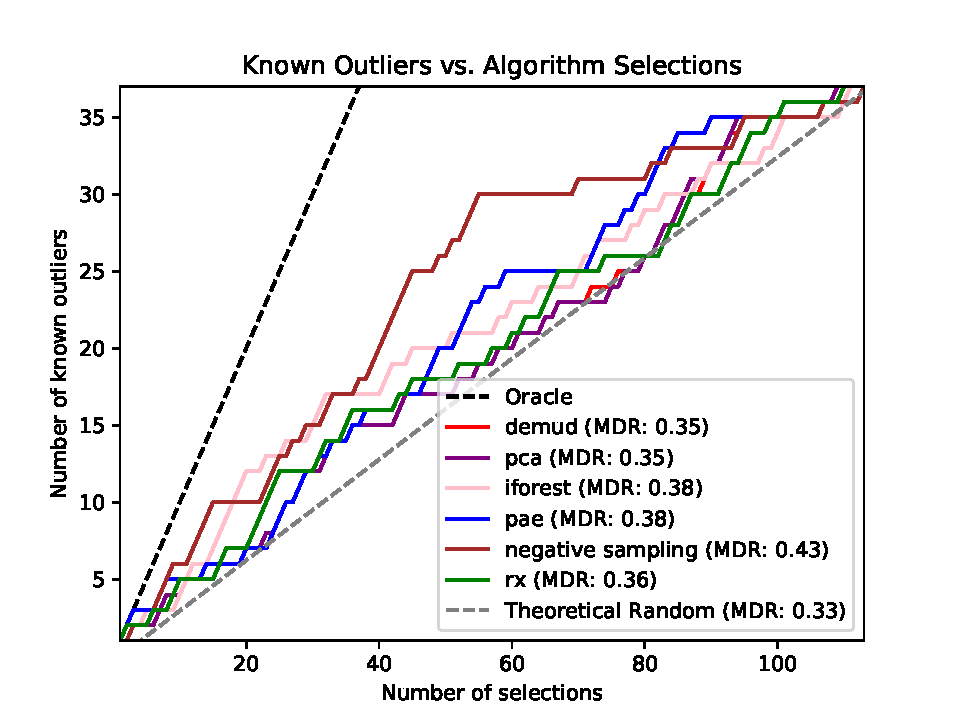
\includegraphics[width=\linewidth]{figures/faw_combined_plot.pdf}
    \caption{Number of known outliers ranked in top $N$ selections for 
    Earth science dataset.}
    \label{fig:faw_results}
\end{figure}

\begin{figure}[h]
    \centering
    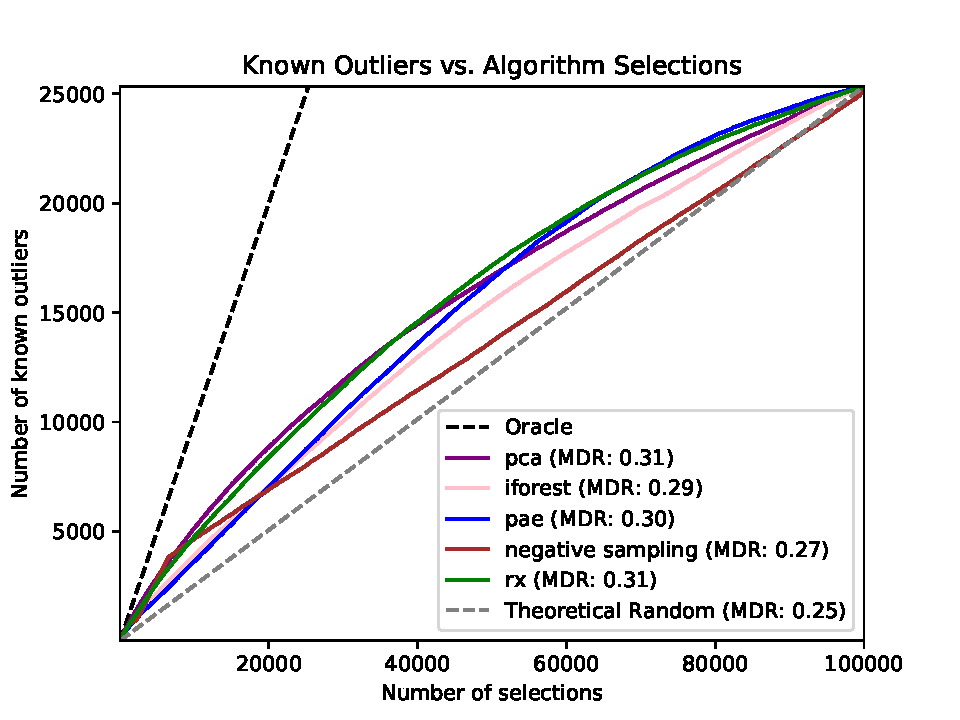
\includegraphics[width=\linewidth]{figures/des_combined_plot.pdf}
    \caption{Number of known outliers ranked in top $N$ selections for 
    the astrophysics (DES) dataset.}
    \label{fig:des_results}
\end{figure}

The experimental setup for each dataset was to fit or train a model for
each ranking algorithm using a larger unlabeled dataset and then apply 
the models to compute the outlier scores for a smaller test dataset for which
labels of known outliers were available (Table \ref{tab:datasets}). 
For each test set, we created a plot of the number of known outliers 
detected out of the top $N$ selections. We also 
reported the Mean Discovery Rate (MDR) in the legend
for each algorithm to give a quantitative comparison across the datasets. We defined MDR as:
\begin{equation}
MDR = \frac{\sum^{N_s}_{i=1} n_i}{\sum^{N_s}_{i=1} s_i}
\end{equation}
where $i \in [1, N_s]$ is the selection index,
 $N_s$ is the total number of selections,
 $s_i$ is the number of selections made up to index $i$,
 and $n_i$ is the number of known outliers (true positives)
among $s_i$ selections.
We also reported the precision at $N=n_{outlier}$ for each test set where
$n_{outlier}$ is the number of known outliers, i.e.,  the precision obtained 
when the number of selections is the same as the total number of outliers. 
Precision at $N$ is the number of known outliers divided by the number of 
selections $N$~\citep{campos2016evaluation}.
Table~\ref{tab:faw_results} compares the precision at $N=n_{outlier}$ for
each dataset and ranking algorithm. 
We calculated a random selection baseline which we refer to as ``Theoretical
Random'' using the expected value of $n_i$ for $i$ random selections:
\begin{align}
\mathbf{E}[n_i, i \in[1, N_s]] &= \frac{\sum^i_{j=0} {n_{outlier}\choose j} {D-n_{outlier}\choose i-j} j}{{D\choose i}} \\
&= \frac{n_{outlier}i}{D}
\end{align}

%\todo{Hannah: Consider merging all three data set discussions since they are
%in one table? with their own figures? The point here isn't really to
%compare algs or data sets but instead to show that we CAN compare
%them, using DORA.}
% We initialized each algorithm with $D_s$ and requested a ranking of
% targets in $D_{s+}$.
%

For the planetary dataset, we found that
the Isolation Forest achieved the highest precision (best outlier
detection) when allowed to select only \num{9} images.
Figure~\ref{fig:planetary_results} shows the complete (cumulative)
outlier detection performance for each algorithm when ranking
all \num{58} target images in $D_{1694-1703}$. We could not
employ RX since the data dimensionality ($64 \times 64 =
4096$) exceeded the data set size. 

For the Earth dataset, negative sampling had the best performance
in both metrics. DEMUD, PCA, and PAE tied for the lowest precision at 
$N=n_{outlier}$ while DEMUD and PCA tied for the lowest
MDR (Figure \ref{fig:faw_results}). We did not evaluate LRX for this time 
series dataset because LRX can only be applied to gridded image or raster 
data types.

For the astrophysics dataset (Figure~\ref{fig:des_results}), DEMUD was omitted due to computational time 
and LRX was omitted as it applies only to image data.  Of the remaining methods, 
PCA achieved the highest precision, following by RX.  Negative sampling 
performs well initially before its performance drops off.  The PAE finds the most outliers 
overall.  

For the MNIST and F-MNIST dataset, PCA and DEMUD tied for the highest
 precision at $N=n_{outlier}$
while DEMUD, PCA, and PAE tied for the highest MDR. Negative sampling had the 
lowest performance in both metrics. 

\section{Discussion}

\begin{figure}
    \centering
    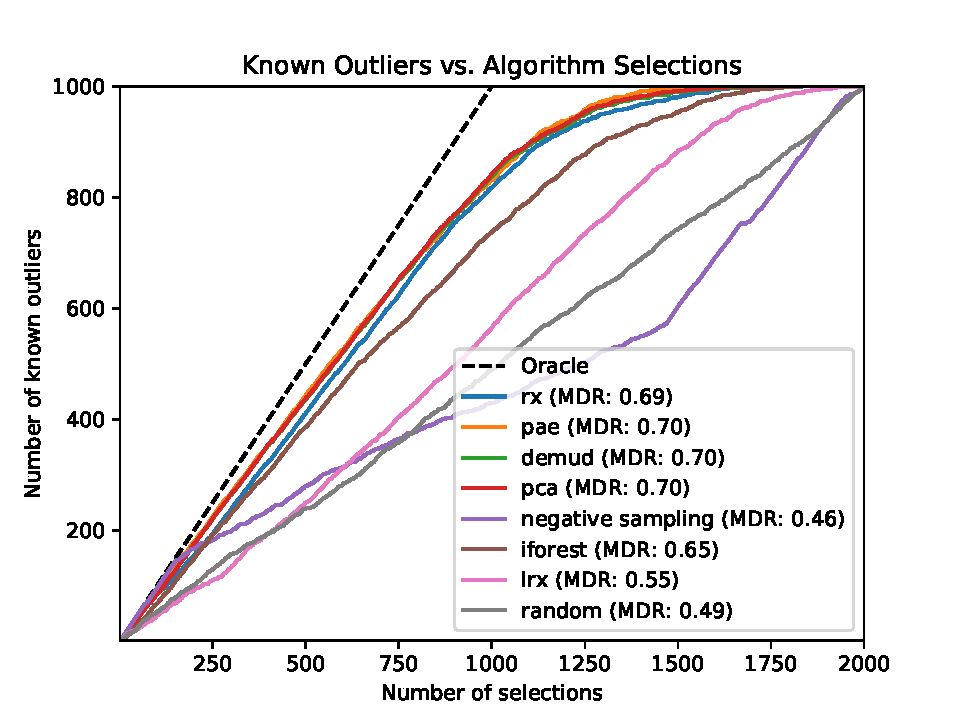
\includegraphics[width=\linewidth]{figures/fmnist_combined_plot.pdf}
    \caption{Number of known outliers ranked in top $N$ selections for 
    F-MNIST dataset.}
    \label{fig:fmnist_results}
\end{figure}

\paragraph{Algorithm performance.} 
No one algorithm  
 had the best performance across all four datasets. PCA had
the best performance for the astrophysics and F-MNIST datasets, 
while negative sampling and isolation forest was best for
the Earth science and planetary datasets respectively. This illustrates
the importance of including a diverse set of algorithms and tools for
easily inter-comparing them in DORA, since the best
algorithm will vary for different datasets. The purpose of this study
was to demonstrate how DORA could be used to facilitate 
outlier detection experiments and compare results across datasets from 
different domains. Thus we did not perform hyperparameter tuning which
could improve results for each dataset; we leave this for future work.
 
\paragraph{Evaluation in outlier detection.} 
Prior work has emphasized
the difficulty of creating standardized metrics for outlier detection that 
represents how models will perform in real world settings while also enabling
intercomparison between datasets~\cite{campos2016evaluation}. We chose two
complementary metrics with this in mind: precision at $N=n_{outliers}$, which
measures the fraction of selections that are known outliers when the number of
selections is equivalent to the number of outliers, and
 Mean Discovery Rate, which measures the fraction of selections that are known outliers on average. 
Designing experiments to evaluate outlier detection methods for real-world
use cases is also difficult because it is difficult, or sometimes impossible, 
to obtain labeled samples of outliers, inliers, or both for evaluation. 
In addition, labels are often subjective or uncertain, 
especially in the case of scientific datasets. For example, a dataset of known
outliers was available for the astrophysics dataset from human annotation
in prior work, but the remainder of samples in the dataset used for evaluation
were not known to be inliers or outliers. This can result in evaluation metrics
 that are deceptively low because unlabeled samples that might actually be
 outliers (as was found to be common in prior work~\cite{wagstaff:des-anom20})
 are counted as false positives. 

\paragraph{Path to deployment.} 
Our goal is for DORA to enable increased application and benefit of
outlier detection methods in real-world scientific use cases. We have 
designed DORA to make it as easy as possible for scientists to apply
algorithms and to compare and interpret their results; users need only
to specify the specifics of their data (e.g., path, data type) in a 
configuration file to start running experiments and seeing results. We will
make DORA publicly available as a pip-installable package to make it
easy to integrate into existing scientific workflows. 
The source code and example datasets used in this study will also be 
open-sourced, enabling DORA to be improved and expanded by the 
machine learning and domain science communities. 
In addition, DORA will be infused into the scientific workflows for the
three use cases we demonstrated results for in this study.
%the use cases from this will also lead to infusion in real scenarios

\section{Conclusion}
The ability to automatically find outliers in large datasets is critical
for a variety of scientific and real-world use cases. 
We presented Domain-agnostic Outlier Ranking Algorithms (DORA),
a configurable pipeline that facilitates application and evaluation of
outlier detection methods in a variety of domains. DORA minimizes the
coding and ML expertise required for domain scientists since users
need only to specify their experiment details in a configuration file
to get results from all available algorithms. This is particularly important
because the experiments for three cross-domain science datasets in this
study showed that no one algorithm performs best for all datasets.
DORA will be publicly accessible as a python package to make it
easy to integrate into existing scientific workflows. 
The will be
open-sourced to enable continued improvement and expansion of DORA
to serve the needs of the science community. The datasets used in this
study will also be public and can serve as real-world benchmarks 
for future outlier detection methods. In future work, we will
continue to improve DORA based on the experience of deploying it in
the workflows of the domain scientists associated with the datasets in
this study and add additional interpretation modules 
including causal inference graphs.

%\section{Acknowledgments}
%We thank the NASA Center Innovation Fund and the NASA Science Mission 
%Directorate (under the NASA Cross-Divisional AI Use Case Demonstration grants)
% for supporting this work.
%
%We thank the UN Food and Agriculture Organization (FAO) and Dr. Ritvik Sahajpal
%(University of Maryland/NASA Harvest) for providing the maize ground
% observation dataset.
% 
% We thank Raymond Francis for analyzing the Navcam rover images to
%identify targets considered to be ``novel'' for evaluating outlier
%detection in the planetary rover scenario.
%
%Part of this research was carried out at the Jet Propulsion
%Laboratory, California Institute of Technology, under a contract with
%the National Aeronautics and Space Administration.

\bibliography{dora_references}

\end{document}

% LocalWords:  tex OOD Eigenbasis DEMUD PCA Xiaoli RX autoencoder al
% LocalWords:  Pimentel mislabeled Liang Böhm wagstaff demud Xiong
% LocalWords:  Storey Hayat des anom Lochner Chiang Zhou Liu Alvera
% LocalWords:  Azcárate Touati Prochaska Kerner kerner PyOD zhao pyod
% LocalWords:  API Umaa Vinay Navcam MNIST FashionMNIST installable
% LocalWords:  dora CIF SMD FAO Pritchard
